\documentclass[11pt]{article}

\usepackage[margin=1in]{geometry}
\usepackage[utf8]{inputenc}
\usepackage[T1]{fontenc}
\usepackage{microtype}
\usepackage{graphicx}
\usepackage{booktabs}
\usepackage{amsmath}
\usepackage{multirow}
\usepackage[numbers,sort&compress]{natbib}
\usepackage[hidelinks]{hyperref}
\usepackage{caption}
\captionsetup{font=small,labelfont=bf}

\newcommand{\harness}[1]{\textsf{#1}}

\title{\textbf{The Harness Tax: Measuring the Token Overhead of\\LLM Coding Harnesses Under a Fixed Model}}
\author{Eishan Lawrence\\\texttt{eishanlawrence5@gmail.com}}
\date{June 2026}

\begin{document}
\maketitle

\begin{abstract}
Benchmarks for LLM-based software engineering overwhelmingly compare \emph{models} while holding the surrounding software fixed. We invert the experiment: we hold the model fixed and compare twelve coding-harness configurations, all driven through a single API gateway, on twelve small Python tasks with deterministic oracles. On tasks that every configuration solves at a near-identical rate, token consumption per solved task spans 46$\times$ on one model and 83$\times$ on a second, unrelated model. The spread decomposes into a fixed per-call \emph{startup tax} (0.7k--24k tokens, a model-independent constant of each harness), turn count, and per-turn context growth: startup tax times turn count predicts cost per solved task with $R^2 = 0.99$ on both models, while context-growth rates occupy a narrow band whose internal ranking does not replicate. Cache-aware accounting reverses several rankings, and we show that a harness's cache-read share is a property of the full harness--gateway--provider path rather than of the harness alone. Two stress extensions probe whether the overhead buys robustness: on ten SWE-bench Lite tasks, four harnesses spanning the cost spectrum resolve exactly the same single task while spending between 0.8M and 15.0M tokens; under 100k tokens of injected irrelevant context, the model itself does not degrade, but harness behavior fractures into five modes (faithful transmission, faithful transmission with task loss, silent truncation, up-front refusal, and crash), of which the silent ones cannot be distinguished from success in the harness's output. For the regimes measured here, the model sets the capability ceiling while the harness sets the price.
\end{abstract}

\section{Introduction}
\label{sec:intro}

A modern AI coding session involves two distinct pieces of software: the language model that produces text, and the \emph{harness}, the CLI tool or agent runtime that wraps the model, assembles its prompts, exposes tools, loops over intermediate results, and applies edits to the user's repository. Public evaluation effort is allocated almost entirely to the first piece. Leaderboards such as SWE-bench~\citep{jimenez2024swebench} rank models under a fixed scaffold, and scaffold papers~\citep{yang2024sweagent,wang2024openhands} report end-to-end resolution rates in which model and harness contributions are confounded. The cost side of the ledger is even less examined: \citet{kapoor2024agents} document that agent evaluations routinely ignore cost entirely, allowing arbitrarily expensive scaffolding to masquerade as capability.

This paper asks a deliberately narrow question: \emph{holding the model fixed, what does the harness itself cost, and is that cost an attribute of the harness or an interaction with the model?} The question matters practically (harness choice is free to change, while model quality is not) and methodologically, because any benchmark that bills harness overhead to the model mismeasures both.

We measure twelve harness configurations on twelve small Python tasks with deterministic pass/fail oracles, routing every configuration through the same API gateway (OpenRouter~\citep{openrouter}) so that all of them face an identical serving substrate. We then repeat the entire experiment on a second, architecturally unrelated model to separate harness-intrinsic effects from model--harness interactions. Three follow-up experiments stress the regime boundaries: a SWE-bench Lite~\citep{jimenez2024swebench} contrast run on hard tasks, a context-injection harm curve with up to 100k tokens of irrelevant material, and a network-level transmission-fidelity probe across all twelve configurations.

\paragraph{Contributions.}
\begin{enumerate}
  \item A controlled, model-factored measurement of harness token overhead: on tasks where capability is saturated, cost per solved task spans 46--83$\times$ across harnesses under a fixed model (Section~\ref{sec:headline}).
  \item A decomposition showing that fixed per-call prompt overhead (``startup tax'') multiplied by turn count, not per-turn context growth, drives the spread: $\log(\text{startup tax} \times \text{turns})$ predicts $\log(\text{cost per solved task})$ with $R^2 = 0.99$ on both models, while context-growth ranks replicate only weakly ($\rho = 0.67$) (Sections~\ref{sec:startup}--\ref{sec:growth}).
  \item Evidence that cache-aware accounting is mandatory, and that the cache-read share is a property of the harness--gateway--provider path: the same gateway yielded 56--85\% cache reads for harnesses speaking its OpenAI-style dialect and near-zero for the one harness speaking its Anthropic-style dialect (Section~\ref{sec:cache}).
  \item A demonstration, on one model, that on tasks beyond that model's capability ceiling an 18$\times$ spread in harness spending purchases identical outcomes (Section~\ref{sec:swe}).
  \item A taxonomy of five harness behaviors under oversized context (faithful, faithful-but-task-losing, silently truncating, refusing, and crashing), established by measuring what each harness actually transmits to the model, and a finding that the model itself is robust at 100k tokens of distractor context even when popular harnesses are not (Sections~\ref{sec:dcurve}--\ref{sec:fidelity}).
\end{enumerate}

All result snapshots, metric implementations, and the figures in this paper are reproducible from the accompanying repository; raw traces are regenerable with the released tooling.\footnote{\url{https://github.com/eishan05/harness-efficiency-bench}}

\section{Related Work}
\label{sec:related}

\paragraph{Agentic software-engineering benchmarks.}
SWE-bench~\citep{jimenez2024swebench} established repository-level issue resolution as the standard capability benchmark; SWE-agent~\citep{yang2024sweagent} showed that the agent--computer interface materially affects resolution rate, and OpenHands~\citep{wang2024openhands} provides an open platform in which scaffolds are compared under fixed models. AgentBench~\citep{liu2024agentbench} evaluates models-as-agents across environments. These efforts vary the model under a fixed scaffold or vary the scaffold under a fixed model to maximize \emph{accuracy}; none isolates the token \emph{overhead} attributable to the scaffold itself, which is our focus. Our SWE-bench contrast run (Section~\ref{sec:swe}) is intentionally the inverse of a leaderboard: the tasks turn out to sit at the model's capability ceiling, so the residual spending differences are pure harness behavior.

\paragraph{Cost-aware evaluation.}
\citet{kapoor2024agents} argue that agent benchmarks must report cost-controlled accuracy, observing that retry-heavy scaffolds dominate leaderboards at unreported expense. We adopt their position and push it one level lower: even at \emph{fixed} accuracy and fixed model, the wrapper alone induces order-of-magnitude cost differences, and cache-read pricing~\citep{gim2024promptcache} changes which wrapper is expensive.

\paragraph{Long-context degradation.}
A substantial literature documents model-side degradation with long or distractor-laden inputs: position effects~\citep{liu2024lost}, reasoning degradation with input length~\citep{levy2024same}, and effective context shorter than advertised~\citep{hsieh2024ruler}. Our harm-curve experiment (Section~\ref{sec:dcurve}) adds a complementary observation: in our setting the \emph{model} tolerated 100k tokens of injected noise when it received them in a single call, while several \emph{harnesses} failed first: by losing the task across turns, truncating silently, refusing, or crashing. Long-context robustness of a deployed system is therefore a property of the harness--model pair, not of the model alone.

\paragraph{Agentic loop designs.}
The looping pattern instantiated by most harnesses descends from ReAct~\citep{yao2023react} and self-refinement approaches~\citep{shinn2023reflexion}. Our results quantify the standing cost of that loop on tasks that do not need it: a single-call harness (Aider~\citep{aider}) solves the same tasks at roughly one tenth the median agentic cost.

\section{Benchmark Design}
\label{sec:design}

\subsection{Harness configurations}
Twelve configurations cover eleven harnesses (\harness{Aider}~\citep{aider}, \harness{Claude Code}~\citep{claudecode}, \harness{Codex CLI}~\citep{codexcli}, \harness{Goose}, \harness{Hermes}, \harness{Kilo}, \harness{Kimi Code}, \harness{Nanobot}, \harness{OpenClaw}, \harness{Opencode}, and \harness{Qwen Code}) plus \harness{Aider} in architect mode. Each runs in an isolated Docker container against a fresh per-task workspace, with credentials pointing at OpenRouter and the same configured model identifier. Aider is a single-call (or two-call, in architect mode) harness; all others implement an agentic observe--act loop with tool use.

\subsection{Tasks and oracles}
The core suite contains twelve small Python-centric tasks (Appendix~\ref{app:tasks}): ten well-specified bug fixes, feature implementations, and file-format migrations, plus two harness-stress tasks that embed the request in noisy or partially conflicting instructions. Every task ships a deterministic oracle (a pytest suite or exact-output check) executed after the harness exits; a task counts as \emph{oracle-solved} only if the oracle passes. The suite is intentionally easy: every configuration solves 11 or 12 of 12 tasks on both models, so cost comparisons are made at approximately matched accuracy rather than across confounded accuracy levels~\citep{kapoor2024agents}.

\subsection{Models and serving}
All traffic flows through OpenRouter, a unified API gateway, so every harness faces the same gateway, the same nominal pricing structure, and the same configured model. Two qualifications matter. First, the gateway routes each request to one of several upstream serving providers unless pinned; we did not pin a provider, and Sections~\ref{sec:cache} and~\ref{sec:threats} examine the consequences. Second, harnesses choose their API dialect: eleven configurations speak the gateway's OpenAI-style \texttt{/chat/completions} endpoint, while Claude Code speaks its Anthropic-style \texttt{/messages} endpoint, which turns out to affect cache behavior (Section~\ref{sec:cache}). The primary model is \texttt{deepseek/deepseek-v4-flash} (a 200k-context model in the DeepSeek line~\citep{deepseek2024v3}); the replication model is \texttt{nvidia/nemotron-3-ultra-550b-a55b:free} (NVIDIA Nemotron line~\citep{nvidia2024nemotron}), chosen to be organizationally unrelated, and free to query so that the replication is reproducible at zero cost.\footnote{No technical report exists for either exact model version; we cite the nearest released report in each model line.} The Nemotron free tier reports no cache-read counts, which itself becomes a finding constraint (Section~\ref{sec:cache}). Each configuration--model pairing was run once; Section~\ref{sec:threats} discusses the single-run design.

\subsection{Metrics}
\label{sec:metrics}
All metrics are computed from per-call token usage recorded in harness traces, cross-checked against gateway-reported billing. Calls billed to a model other than the dominant configured model (auxiliary traffic, Section~\ref{sec:aux}) are excluded from per-call structural metrics but included in totals.

\paragraph{A: Startup tax.} The input-token count of the first model call minus the token count of the rendered user prompt: the fixed payload (system prompt, tool schemas, environment preamble) the harness attaches before any work occurs. Because models are stateless, this payload is retransmitted on every call; its effective cost is the tax times the turn count.

\paragraph{B: Context growth rate.} The least-squares slope of input tokens versus call index over the dominant monotone thread of the conversation, with a divergence guard that flags runs where the slope and the median adjacent-call delta disagree by more than 2$\times$ (indicating front-loaded or compaction-distorted growth rather than steady accumulation). Aider's single-call runs admit no slope, and the architect variant's two-call runs yield a line through two points rather than a growth rate; both are excluded from cross-model comparisons of B.

\paragraph{Turn count.} The number of model calls a run makes to the configured task model (auxiliary helper calls to other models, Section~\ref{sec:aux}, excluded). We report the per-task median.

\paragraph{C: Token--solve efficiency.} Total billed tokens divided by oracle-solved tasks. A \emph{cache-discounted} variant weights cache-read input tokens at $0.1\times$, matching the common provider discount for cached prefixes~\citep{gim2024promptcache}.

\paragraph{D: Context-bloat harm curve.} The suite is re-run with 20k, 50k, and 100k tokens of irrelevant log noise prepended to each task prompt; we track solve rate and cost as functions of injected volume.

\paragraph{Transmission fidelity.} For the 100k injection level, the maximum single-call input-token count divided by the rendered prompt's token count. Values near 1 indicate the harness transmitted the payload; values far below 1 indicate it silently did not. The metric measures single-call transmission: a harness that chunked the payload across several calls would score low while being faithful in aggregate. We verified from per-call traces that no low-scoring harness chunks; their call sizes start at a fixed window and grow only by ordinary per-turn accretion (Section~\ref{sec:fidelity}).

\paragraph{Cross-model stability.} For each metric we compute Spearman rank correlation~\citep{spearman1904} between the two models across the twelve configurations. A metric that is a property of harness software should replicate in rank; a model--harness interaction need not.

\section{Results}
\label{sec:results}

\subsection{Headline: a 46--83$\times$ spread at matched accuracy}
\label{sec:headline}

Table~\ref{tab:main} and Figure~\ref{fig:cost} present the core result. With the model, tasks, gateway, and (approximately) accuracy held fixed, tokens per oracle-solved task range from 4{,}125 (\harness{Aider} architect) to 190{,}778 (\harness{OpenClaw}) on DeepSeek V4 Flash, a 46$\times$ spread, and from 3{,}522 to 292{,}281 on Nemotron 3 Ultra, an 83$\times$ spread. The ordering is nearly identical across the two models (one adjacent transposition); the spread is a property of the harness software, not of any model quirk.

\begin{table}[t]
\centering
\small
\caption{Core results on the 12-task suite. A = startup tax (tokens); turns = median model calls per task (DeepSeek); C = tokens per oracle-solved task; C$_{0.1}$ = cache-discounted C (cache reads at $0.1\times$); cached = share of total billed tokens that were cache reads (DeepSeek run; the Nemotron free tier reports no caching). Solved is out of 12. Rows ordered by C on DeepSeek.}
\label{tab:main}
\begin{tabular}{l rr r rr r r cc}
\toprule
 & \multicolumn{2}{c}{A (tokens)} & turns & \multicolumn{2}{c}{C (tokens/solve)} & C$_{0.1}$ & cached & \multicolumn{2}{c}{solved} \\
\cmidrule(lr){2-3}\cmidrule(lr){4-4}\cmidrule(lr){5-6}\cmidrule(lr){7-7}\cmidrule(lr){8-8}\cmidrule(lr){9-10}
Harness & DS & NM & DS & DS & NM & DS & DS & DS & NM \\
\midrule
Aider (architect) & 708 & 741 & 2 & 4{,}125 & 3{,}522 & 4{,}125 & 0\% & 11 & 11 \\
Aider             & 3{,}044 & 3{,}069 & 1 & 5{,}031 & 4{,}114 & 5{,}031 & 0\% & 11 & 11 \\
Hermes            & 2{,}574 & 2{,}542 & 7 & 30{,}454 & 34{,}320 & 16{,}045 & 53\% & 12 & 12 \\
Claude Code       & 4{,}512 & 4{,}613 & 9 & 51{,}820 & 54{,}580 & 51{,}793 & 0\% & 12 & 12 \\
Goose             & 3{,}920 & 4{,}435 & 10 & 55{,}674 & 61{,}865 & 21{,}594 & 68\% & 12 & 11 \\
Nanobot           & 8{,}499 & 9{,}691 & 7 & 73{,}512 & 84{,}488 & 18{,}897 & 83\% & 12 & 12 \\
Opencode          & 8{,}366 & 8{,}672 & 8.5 & 79{,}634 & 71{,}864 & 25{,}068 & 76\% & 12 & 12 \\
Codex             & 8{,}038 & 8{,}359 & 8.5 & 84{,}794 & 89{,}643 & 26{,}291 & 77\% & 12 & 11 \\
Kimi Code         & 16{,}041 & 16{,}510 & 6 & 105{,}185 & 116{,}047 & 53{,}489 & 55\% & 12 & 12 \\
Kilo              & 14{,}477 & 14{,}877 & 9.5 & 119{,}316 & 120{,}407 & 49{,}072 & 65\% & 12 & 12 \\
Qwen Code         & 21{,}408 & 19{,}031 & 8.5 & 181{,}662 & 140{,}996 & 71{,}204 & 68\% & 12 & 12 \\
OpenClaw          & 23{,}682 & 29{,}035 & 7 & 190{,}778 & 292{,}281 & 71{,}095 & 70\% & 11 & 11 \\
\bottomrule
\end{tabular}
\end{table}

\begin{figure}[t]
\centering
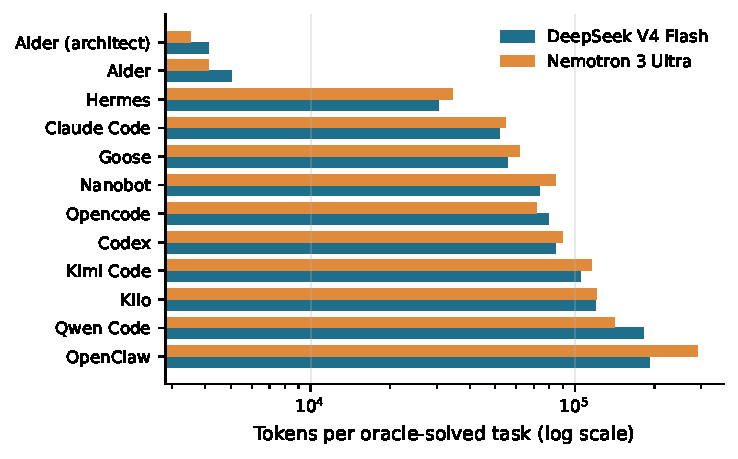
\includegraphics[width=0.78\linewidth]{figures/fig_cost.pdf}
\caption{Tokens per oracle-solved task across twelve harness configurations on two unrelated models. Note the logarithmic axis: the spread is 46$\times$ (DeepSeek) and 83$\times$ (Nemotron), and the ordering is nearly preserved across models.}
\label{fig:cost}
\end{figure}

\subsection{The startup tax is a software constant}
\label{sec:startup}

The fixed prompt overhead a harness attaches before any task content ranges from 708 tokens (\harness{Aider} architect) to 23{,}682 tokens (\harness{OpenClaw}): a 33$\times$ spread before any work has started. Per-harness values reproduce across the two models to within a few percent (Figure~\ref{fig:startup}), and the cross-model rank correlation is exactly $\rho = 1.000$ (Table~\ref{tab:spearman}). We read the perfect rank agreement as a manipulation check rather than a discovery: the same binary emits the same prompt bytes regardless of the model behind the gateway, and only the tokenizer differs. The startup tax behaves like a binary's file size: a constant of the software.

Its importance is multiplicative rather than additive. Because each model call retransmits the full conversation, a harness with a 24k-token floor that takes 15 turns has spent roughly 360k input tokens on scaffolding alone. The decomposition is quantitative: startup tax alone rank-correlates with cost per solved task at $\rho = 0.951$ on DeepSeek, and combining it with turn count, $\log(\text{A} \times \text{mean turns})$ predicts $\log(\text{C})$ with $R^2 = 0.990$ on DeepSeek and $0.992$ on Nemotron (Spearman 0.979 and 0.986). Turn counts contribute little of the variance on these tasks because every looping harness lands in a narrow band of 6--10 median turns (Table~\ref{tab:main}); the floor each turn re-carries is what separates the harnesses.

\begin{figure}[t]
\centering
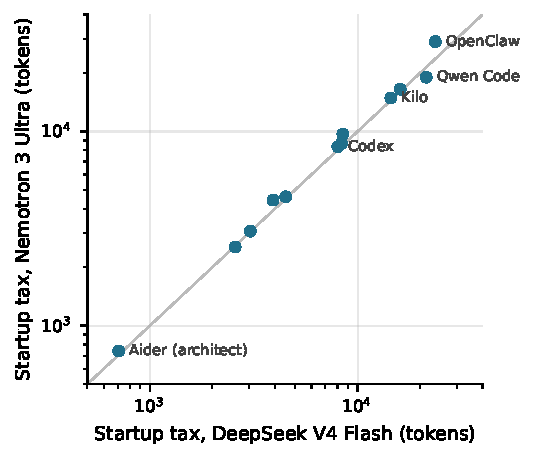
\includegraphics[width=0.5\linewidth]{figures/fig_startup.pdf}
\caption{Startup tax measured independently on two models (log--log). Points lie on the identity line: the harness's fixed prompt overhead is model-independent, with cross-model Spearman $\rho = 1.000$.}
\label{fig:startup}
\end{figure}

\subsection{Context growth does not separate harnesses}
\label{sec:growth}

A natural hypothesis is that expensive harnesses are those whose conversations balloon fastest. The data reject this. Every looping harness grew its context within a narrow band of roughly 230--560 tokens per turn on DeepSeek, and the cross-model rank correlation of growth rates is only $\rho = 0.673$ ($n = 10$, Table~\ref{tab:spearman}): the \emph{band} replicates, but the ranking within it replicates only weakly. With one run per pairing we cannot attribute the residual to run-to-run noise versus a genuine model--harness interaction; either way, within-band differences carry no cost signal at this scale. Turn counts behave similarly: the 6--10-turn band reproduces on both models while ranks within it correlate at only $\rho = 0.664$. What separates harnesses is the size of the floor each turn re-carries (Section~\ref{sec:startup}). For harness builders, the actionable ordering is: reduce the prompt floor and reduce turns before optimizing context accretion.

\begin{table}[t]
\centering
\small
\caption{Cross-model rank stability (Spearman $\rho$, DeepSeek vs.\ Nemotron, across harness configurations). Startup tax and solve efficiency are properties of the harness software; turn-count and context-growth ranks replicate only weakly. B excludes Aider (no slope) and Aider architect (two-point slope).}
\label{tab:spearman}
\begin{tabular}{l c c}
\toprule
Metric & $\rho$ & $n$ \\
\midrule
A: startup tax & 1.000 & 12 \\
C: tokens per oracle-solved task & 0.993 & 12 \\
turns: median model calls per task & 0.664 & 12 \\
B: context growth rate & 0.673 & 10 \\
\bottomrule
\end{tabular}
\end{table}

\subsection{Cache-aware accounting reverses rankings}
\label{sec:cache}

Raw token counts misprice harnesses that are cache-friendly. On the DeepSeek run, \harness{Codex} consumed 84{,}794 raw tokens per solved task, nominally among the most expensive, but 77\% of its billed tokens were cache reads, which providers typically price at one tenth of the uncached rate~\citep{gim2024promptcache}. Under cache-discounted accounting (Figure~\ref{fig:cache}), \harness{Codex} costs 26{,}291 effective tokens per solved task, \emph{less than half} of \harness{Claude Code}'s 51{,}793, despite Claude Code using half the raw tokens; Claude Code's traffic on this serving path registered essentially no cache reads (0.1\% of input). Similar reversals affect \harness{Goose}, \harness{Nanobot}, and \harness{Opencode}, all of which drop 60--75\% of their nominal cost under realistic pricing.

Claude Code's zero share is not a property of its prompts. It is the only configuration that speaks the gateway's Anthropic-style \texttt{/messages} dialect; the eleven OpenAI-dialect configurations earned 56--85\% cache reads on the same gateway and model. Gateway generation records show Claude Code's calls landing consecutively on a single upstream provider with strictly growing, prefix-shared prompts and zero cache reads throughout, while a controlled probe found that the same provider \emph{does} serve cache reads for identical prefixes submitted through \texttt{/chat/completions}, and that the \texttt{/messages} translation produced none when pinned to a caching provider. The cache-read share is therefore a property of the harness--gateway--provider path, including the API dialect on the wire, not of the harness alone.

Three consequences follow. First, raw token dashboards are not comparable across harnesses; the cached share must be reported alongside any count. Second, prefix stability is necessary but not sufficient: re-sending an identical prefix every turn is the access pattern prompt caching rewards, but the serving path must also propagate it, and one popular dialect translation on this gateway did not. Third, the discount is contingent on the path end to end: the Nemotron free tier reported no cache reads at all, so the discounted and raw rankings coincide there.

\begin{figure}[t]
\centering
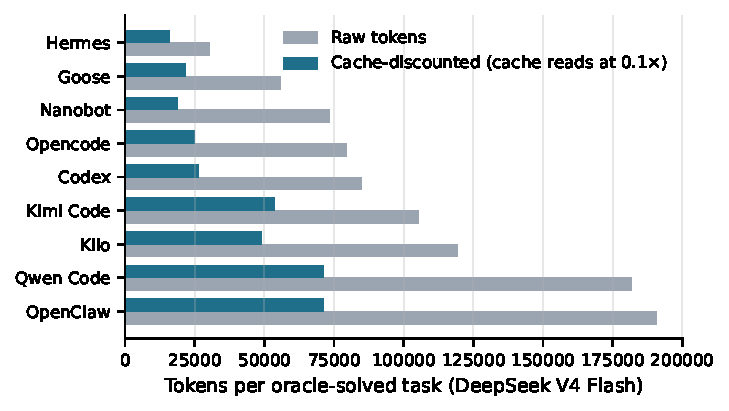
\includegraphics[width=0.72\linewidth]{figures/fig_cache.pdf}
\caption{Raw versus cache-discounted tokens per solved task (DeepSeek run; harnesses with measurable cache traffic). Discounting cache reads at $0.1\times$ collapses most of the apparent cost of cache-friendly harnesses and reverses several pairwise rankings.}
\label{fig:cache}
\end{figure}

\subsection{The cheapest configuration is the one without a loop}
\label{sec:oneshot}

\harness{Aider} solved 11 of 12 tasks at roughly 4--5k tokens per solve on both models, an order of magnitude below the median agentic harness, by making a single model call per task: file content in, diff out. The agentic observe--act loop~\citep{yao2023react} is a cost multiplier that pays for itself only when a task requires exploration or iteration; on small, fully specified edits, the loop largely re-derives facts a single call could assume. Matching harness style to task size is the largest single cost lever in this dataset, exceeding any plausible model-pricing difference.

\subsection{Auxiliary model traffic}
\label{sec:aux}

Trace-level accounting attributed calls per billed model and surfaced a behavior not visible in the configuration surface: two harnesses, \harness{Kilo} and \harness{Opencode}, routed a fixed set of helper calls (e.g., title or summary generation) to \texttt{anthropic/claude-4.5-haiku} rather than the configured model: 16{,}366 and 8{,}170 input tokens per batch respectively, reproduced to the token across both primary models. The volumes are economically negligible, and the behavior may well be documented by the vendors; the observation is that the configured model and the models on the wire can differ, which is material for users with data-routing constraints and is visible only at the trace layer. These calls are excluded from structural metrics (A, B) and retained in totals (C).

\subsection{On hard tasks, spending diverges and outcomes do not}
\label{sec:swe}

To test whether heavyweight scaffolding earns its overhead on hard problems, four harnesses spanning the cost spectrum (\harness{Aider}, \harness{Claude Code}, \harness{Codex}, \harness{Kilo}) ran ten SWE-bench Lite~\citep{jimenez2024swebench} tasks under generous wall-clock and budget limits, with DeepSeek V4 Flash as the model. The ten tasks (Appendix~\ref{app:swetasks}) were selected for repository diversity and evaluation-infrastructure cost, not difficulty. Every harness resolved exactly one task of ten, \emph{the same task} (\texttt{pytest-dev\_\_pytest-5227}), while total spending ranged from 0.82M tokens (\harness{Aider}) through 5.27M (\harness{Claude Code}) and 12.33M (\harness{Kilo}) to 14.96M (\harness{Codex}): an 18$\times$ spread purchasing identical outcomes (Figure~\ref{fig:swe}). The failures are not for want of producing output: measured from the evaluator's patch payload, \harness{Claude Code}, \harness{Codex}, and \harness{Kilo} each submitted a non-empty candidate patch on nine of ten tasks (\harness{Aider} on seven of ten); the patches simply do not resolve the issues.

The reading is that these tasks sit at or beyond this model's capability ceiling, and on the evidence here scaffolding does not raise that ceiling. The finding is established for one model; a stronger model might give heavyweight scaffolds headroom (Section~\ref{sec:threats}). It is consistent with scaffold comparisons under fixed models showing bounded scaffold effects~\citep{yang2024sweagent,wang2024openhands}, but sharper: at the ceiling, the marginal value of scaffolding is zero while its marginal cost spans an order of magnitude. None of the four harnesses detected that it was at a ceiling; the expensive loops spent their budgets circling it.

\begin{figure}[t]
\centering
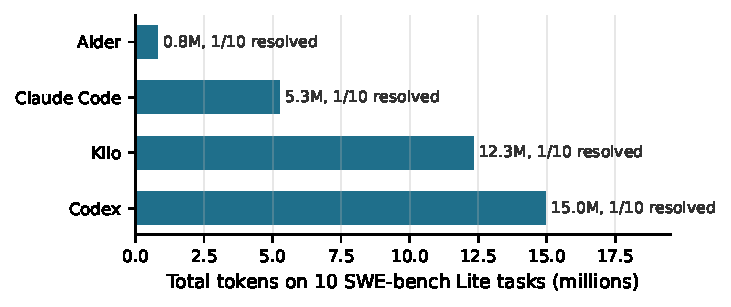
\includegraphics[width=0.7\linewidth]{figures/fig_swe.pdf}
\caption{SWE-bench Lite contrast run (10 curated tasks, DeepSeek V4 Flash). All four harnesses resolve exactly the same single task; spending spans 18$\times$.}
\label{fig:swe}
\end{figure}

\subsection{The harm curve: the model survives 100k of noise; harnesses vary}
\label{sec:dcurve}

The context-bloat experiment prepends 20k--100k tokens of irrelevant log noise to each task prompt for the same four harnesses (Figure~\ref{fig:dcurve}). Four distinct behaviors emerge.

\textbf{The model does not rot at 100k.} \harness{Aider} passes the entire 100k payload to the model in one call and still solves 12/12. Whatever long-context degradation exists for this model on these tasks~\citep{liu2024lost,levy2024same}, it is not the binding constraint at 100k tokens.

\textbf{\harness{Claude Code} collapses at 100k.} Perfect through 50k, it falls to 2/12 at 100k despite \emph{faithfully transmitting} the payload (fidelity $\approx$ 1.05). Runs end after a few calls with no edits: the failure is in the harness's multi-turn context management, not in the model, since the same model solved the same contaminated tasks 12/12 under Aider.

\textbf{\harness{Codex} is faithful and robust, at full price.} It re-transmits the complete payload every turn and stays at 12/12 through 100k, paying payload $\times$ turns: the 100k injection turns an 82k-token suite-average task into a 909k-token one, an 11$\times$ cost increase spent entirely on noise.

\textbf{\harness{Kilo} appears robust by not reading the input.} Its curve is flat in both solve rate and cost because it silently truncates the prompt: roughly 13.5k of the 100k tokens reached the model (fidelity 0.17). The injected noise precedes the task text in the rendered prompt, so a window that retains the prompt's tail keeps the task, and the per-call traces match exactly that: every task call starts at a fixed $\approx$13.5k-token window and grows only by ordinary per-turn accretion. The tasks pass because the retained tail happens to contain the task; nothing in the harness's output distinguishes these runs from ones in which the window would exclude it, so the failure mode is latent rather than absent.

\begin{figure}[t]
\centering
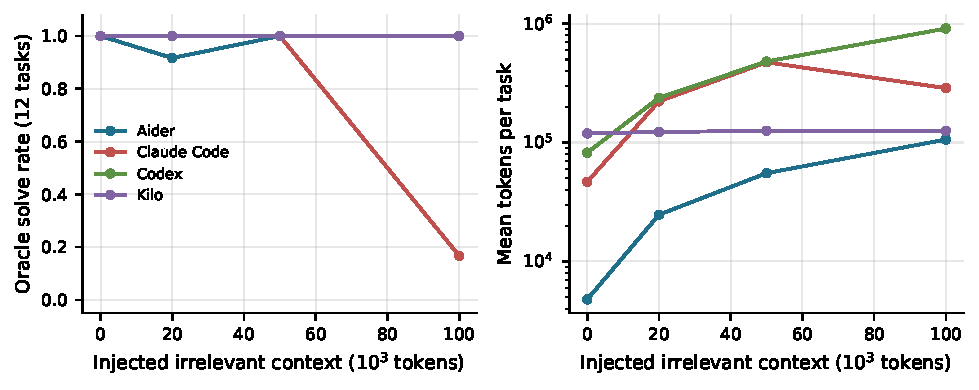
\includegraphics[width=0.98\linewidth]{figures/fig_dcurve.pdf}
\caption{Context-bloat harm curve (DeepSeek V4 Flash, 12 tasks per point). Left: oracle solve rate versus injected irrelevant context. Right: mean tokens per task (log scale). Kilo's flat curves are an artifact of silent truncation (Section~\ref{sec:fidelity}); Codex's cost curve shows the price of faithful retransmission.}
\label{fig:dcurve}
\end{figure}

\subsection{Transmission fidelity: five behaviors, the silent ones invisible from output}
\label{sec:fidelity}

Prompted by Kilo's flat curve, we probed all twelve configurations at the 100k level on the full 12-task suite and measured, from per-call usage, the fraction of the rendered prompt each harness actually transmitted (Figure~\ref{fig:fidelity}; values are per-configuration medians over the 12 tasks). The configurations partition into five classes:

\begin{enumerate}
  \item \textbf{Faithful and robust} (7 of 12): \harness{Aider} (1.03), \harness{Aider} architect (1.01), \harness{Codex} (1.11), \harness{Goose} (1.07), \harness{Hermes} (1.05), \harness{Nanobot} (1.11), \harness{Qwen Code} (1.25) transmit the full payload (ratios above 1 reflect harness framing plus per-turn accretion on top of the payload) and solve 10--12 of the 12 probe tasks.
  \item \textbf{Faithful but loses the task}: \harness{Claude Code} (1.05) transmits everything, then fails 10 of 12 tasks (Section~\ref{sec:dcurve}).
  \item \textbf{Silent truncation} (2 of 12): \harness{Kilo} (0.17) and \harness{Opencode} (0.11) drop 83--89\% of the prompt without notice and ``solve'' 11--12 tasks anyway.
  \item \textbf{Loud refusal}: \harness{OpenClaw} detects the oversize input up front, makes zero model calls on all twelve tasks, and instructs the user to switch models. Unhelpful, but honest.
  \item \textbf{Crash}: \harness{Kimi Code} terminates with an unhandled internal error (a history-compaction failure) on all twelve tasks before completing any.
\end{enumerate}

Critically, classes 1, 3 and (at moderate sizes) 2 are indistinguishable from the harness's user-facing output: ``the task passed'' is consistent with the harness having read all, or one tenth, of what the user supplied. Transmission fidelity is measurable only at the usage/trace layer, which argues for its inclusion in any harness evaluation, and for treating long-context robustness claims about deployed tools~\citep{hsieh2024ruler} as claims about the harness--model \emph{system}.

\begin{figure}[t]
\centering
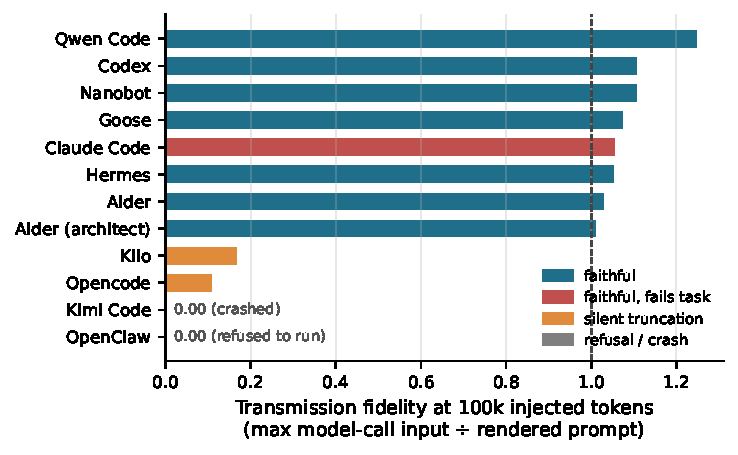
\includegraphics[width=0.74\linewidth]{figures/fig_fidelity.pdf}
\caption{Transmission fidelity at 100k injected tokens for all twelve configurations (median over the 12-task suite): the largest single-call input divided by the rendered prompt size. Seven harnesses transmit faithfully; two silently truncate; one refuses; one crashes; one transmits faithfully and then fails the tasks.}
\label{fig:fidelity}
\end{figure}

\section{Discussion}
\label{sec:discussion}

\paragraph{The model sets the ceiling; the harness sets the price.}
Across all four experiments a single division of labor recurs. Capability saturates with the model: on easy tasks everyone solves everything, on hard tasks everyone solves the same single task, and under 100k of noise the model itself is unimpaired. Cost, by contrast, is set almost entirely by the harness: its fixed prompt floor, its turn count, its cache friendliness, and its context-handling policy. Because the harness is the component a user can change freely, the 46--83$\times$ spread measured here is, in effect, the largest free parameter in the cost of AI-assisted coding; no current model-to-model price difference approaches it.

\paragraph{Implications for users.}
For small, well-specified tasks, a single-call harness pockets roughly 10$\times$ over the agentic median. Token dashboards should never be compared across harnesses without the cached share. Users with data-governance constraints should verify which models appear on the wire, not which model was configured.

\paragraph{Implications for harness builders.}
The leverage ordering implied by the data is: (i) reduce the prompt floor, since it is paid every turn; (ii) reduce turns; (iii) keep the retransmitted prefix byte-stable and verify that the serving path actually awards cache reads for it, since one popular dialect translation on our gateway did not; (iv) make context-overflow behavior explicit, since of the five observed behaviors only loud refusal and faithful transmission preserve the user's mental model of what the tool did; and (v) consider ceiling detection: all four harnesses on SWE-bench spent 0.8--15M tokens failing to notice that additional iterations were not improving a fixed outcome.

\paragraph{Implications for benchmark design.}
Harness overhead is large enough to confound model benchmarks that do not factor it out, and harness rankings are unstable under cache-aware repricing. Cost-controlled evaluation~\citep{kapoor2024agents} should therefore stratify by (model, harness) pairs, report cached and uncached tokens separately, and, given Section~\ref{sec:fidelity}, verify at the trace layer that the evaluated system actually transmitted the benchmark inputs.

\section{Threats to Validity}
\label{sec:threats}

\paragraph{Single run per pairing.} The core grid was executed once per configuration--model pair. We mitigate by replicating the full grid on a second, unrelated model: quantities that reproduce there with $\rho \ge 0.99$ (startup tax, solve efficiency) are unlikely to be run noise, while we explicitly down-weight the metrics that replicated only weakly (context-growth and turn-count ranks). Within-condition variance remains uncharacterized.

\paragraph{Serving path.} The gateway routes each request to one of several upstream providers (we observed at least five distinct providers across the batches), and we did not pin one. Cache findings in Section~\ref{sec:cache} are therefore claims about this gateway's serving paths, supported by per-call generation records and a controlled endpoint probe, not about any provider in isolation. The free-tier Nemotron endpoint adds further unknowns (quantization, sampling configuration, undisclosed limits) beyond its missing cache-read counts.

\paragraph{Task scale and selection.} The core tasks are small, single-file Python edits; the 46--83$\times$ spread is established in that regime. The SWE-bench and harm-curve extensions cover four harnesses and one model, so those findings are held with correspondingly less generality. A frontier model might give heavyweight scaffolds more headroom on hard tasks; that experiment was outside our budget.

\paragraph{Usage accounting.} Token counts derive from harness-reported and gateway-reported usage, which we cross-checked for consistency; the cache-discount factor of $0.1\times$ is a market-typical convention rather than a universal price, and we do not model the cache-write surcharges some providers levy. The transmission-fidelity metric depends on provider-reported input token counts being honest, which the agreement between Aider's fidelity ($\approx 1.03$) and its known single-call design supports.

\paragraph{Harness versions.} Harnesses evolve quickly; all measurements are snapshots of specific containerized versions (pinned in the repository). The claim is not that any vendor's current release behaves identically, but that the \emph{measurement framework} (startup tax, cache-aware efficiency, harm curves, transmission fidelity) separates harnesses on axes that raw leaderboards do not.

\section{Conclusion}
\label{sec:conclusion}

We measured what the wrapper costs. Holding the model, tasks, and gateway fixed, twelve coding-harness configurations differed by 46--83$\times$ in tokens per solved task, with the spread driven by a model-independent per-call prompt floor multiplied by turn count ($R^2 = 0.99$ on both models), materially repriced by cache-aware accounting, and unredeemed on tasks beyond the model's capability ceiling, where an 18$\times$ spending spread bought identical outcomes. Under bloated inputs, harness behavior, not model behavior, fractured into five modes, one of which (silent truncation, observed in two harnesses) misrepresents what the model was shown while reporting success. For the regimes measured, the conclusion is compact: the model supplies the capability, the harness sets the price, and the price varies by nearly two orders of magnitude among tools that present themselves as interchangeable.

\paragraph{Reproducibility.} All result snapshots, metric code, figure-generation scripts, and the harness/task manifests are available at \url{https://github.com/eishan05/harness-efficiency-bench}; raw traces are regenerable with the released tooling. The replication batch uses a free-tier model and can be reproduced at zero API cost.

\bibliographystyle{unsrtnat}
\bibliography{refs}

\appendix

\section{Task Suite}
\label{app:tasks}

The twelve score-facing tasks, each with a deterministic oracle:

\begin{table}[h]
\centering
\small
\begin{tabular}{l l}
\toprule
Task & Description \\
\midrule
\texttt{python-fix-calculator} & Fix arithmetic bugs in a small calculator module \\
\texttt{python-cache-ttl-lru} & Implement a TTL-aware LRU cache \\
\texttt{python-cli-subcommands} & Add subcommands to an argparse CLI \\
\texttt{python-csv-ledger-reconcile} & Reconcile two CSV transaction ledgers \\
\texttt{python-datetime-windowing} & Implement time-window bucketing logic \\
\texttt{python-json-config-migration} & Migrate a JSON config across schema versions \\
\texttt{python-markdown-link-normalizer} & Normalize link syntax in Markdown files \\
\texttt{python-path-safety} & Harden path handling against traversal \\
\texttt{python-plugin-registry} & Implement a plugin registration mechanism \\
\texttt{toy-write-file} & Write a specified file with exact contents \\
\texttt{harness-stress-log-triage} & Extract a fix request from noisy log output \\
\texttt{harness-stress-conflicting-specs} & Resolve partially conflicting instructions \\
\bottomrule
\end{tabular}
\caption{Score-facing task suite. Oracles are pytest suites or exact-output checks executed after the harness exits.}
\label{tab:tasks}
\end{table}

\section{SWE-bench Lite Contrast Tasks}
\label{app:swetasks}

The ten SWE-bench Lite instances used in Section~\ref{sec:swe} were selected for repository diversity (two instances each from Django, SymPy, Matplotlib, pytest, and xarray) and to reuse repo/version families so that evaluation Docker image pulls and builds stay manageable; difficulty played no role in selection. The instances: \texttt{django\_\_django-11905}, \texttt{django\_\_django-12308}, \texttt{matplotlib\_\_matplotlib-23913}, \texttt{matplotlib\_\_matplotlib-24334}, \texttt{pydata\_\_xarray-3364}, \texttt{pydata\_\_xarray-4248}, \texttt{pytest-dev\_\_pytest-5221}, \texttt{pytest-dev\_\_pytest-5227}, \texttt{sympy\_\_sympy-13146}, \texttt{sympy\_\_sympy-14308}.

\section{Context Growth Detail}
\label{app:growth}

Per-turn context growth on DeepSeek V4 Flash ranged from 232 tokens/turn (\harness{OpenClaw}) to 557 tokens/turn (\harness{Kilo}) across the ten looping configurations; \harness{Aider}'s single-call design yields no growth slope, and the architect variant's two-call runs are excluded because a line through two points is not a growth rate. The cross-model Spearman correlation of these slopes is 0.673 ($n = 10$): the few-hundred-tokens-per-turn band is reproducible, but rankings within it replicate only weakly, and we therefore assign within-band differences no cost significance. A divergence guard comparing the fitted slope against the median adjacent-call delta flagged no qualifying run in the core batches as artifactual; mild divergence ratios (2--3$\times$) corresponded to front-loaded growth patterns rather than measurement error.

\end{document}
